\documentclass{article}
\usepackage{graphicx} % Required for inserting images
\usepackage{blindtext}
\usepackage{hyperref}
\usepackage{cite}




\author{Riccardo Dal Cero}
\date{August 2023}

\title{Final Report Research Assistentship}
\author{Riccardo Dal Cero}

\begin{document}
\maketitle

\begin{abstract}

In the dynamic realm of AI-powered communication tools and the growing significance of official language in public discourse, my research venture aimed to investigate the influence of White House speeches on economic and financial variables. Through harnessing the capabilities of sentiment analysis AI models and grammar analysis, my objective was to extract valuable economic narratives from White House press briefings and joint press conferences.
 
The project's trajectory encompassed pivotal stages, ranging from meticulous data collection and preprocessing to sentiment analysis, grammar analysis, and advanced statistical modeling utilizing techniques like Structural Vector Autoregression (SVAR) and Vector Autoregression (VAR) models. My role as a research assistant (RA) entailed steering each of these stages, entailing responsibilities spanning data management, NLP analysis, sentiment analysis employing pre-trained models like BERT, and working with programming languages such as Python, R, and MATLAB.
 
Through scrupulous collection and organization of speech texts, I cultivated an extensive and structured corpus conducive for analysis. Employing data preprocessing strategies, I shaped meaningful time-series variables encapsulating key facets of White House briefings. Sentiment analysis offered a quantifiable assessment of emotional expressions, while grammar analysis granted illuminating insights into linguistic attributes embedded in the speeches.
 
The statistical modeling phase furnished a rigorous examination of the interplay between speech sentiment, media dynamics, and financial market behavior. Leaning on advanced econometric models, I probed the latent determinants of uncertainty policy indices and their ripple effects on economic metrics.
 
The course of this endeavor enabled me to cultivate a diverse skill set, spanning data management, NLP analysis, sentiment analysis, and statistical modeling. Gaining hands-on familiarity with intricate research projects and proficiency in programming languages significantly augmented my competencies.
 
While the project's path revealed salient strengths in its comprehensive approach and systematic analyses, discerning scrutiny also unveiled potential avenues for enhancement. Enriching grammar analysis through incorporation of additional linguistic dimensions and exploring alternative AI models for sentiment analysis could unlock deeper insights into language dynamics. Addressing concerns regarding endogeneity within statistical models and accommodating shifting contexts would enhance the robustness of the research framework.
 
In summation, this endeavor holds the promise of illuminating the intricate interplay among official language, media dynamics, and financial market conduct, thereby furnishing invaluable insights for policymakers, scholars, and the wider public. The findings resonate with a broader comprehension of how language weaves into economic narratives, providing a compass for informed decision-making in an era marked by volatility and evolving communication technologies.

\end{abstract}
\newpage
\section{Introduction}

This report provides an overview of a research project that focuses on using NLP AI techniques to extract economic
narratives from White House speeches. The project aims to analyze the influence of political discourse on media dynamics
and the financial market. This repository contains the code and resources used throughout the project, organized into
several folders: \texttt{Code\_From Download to Dataset}, \texttt{Data}, \texttt{Exploring\_dataset}, and
\texttt{Literature review}.

\subsection{General Description of the purpose of the research}

The research project falls within the social sciences discipline (statistical modelling, finance) and is centered around
the analysis of political communication, media dynamics, and market behavior. The primary objective is to understand how
White House speeches influence the media and subsequently impact the financial market. By applying sentiment analysis AI
models and grammar analysis techniques, the project aims to extract valuable insights from the speeches and investigate
their effects on market sentiment.
\par
In an era where AI tools are capable of generating text and mimicking human communication, public authorities worldwide face the challenge of combating misinformation and effectively disseminating their messages to the broader public. Thus, understanding the impact of official language becomes crucial.
\par
The primary aim of this project is to collect and leverage daily White House (WH) press briefings for empirical text analysis, investigating their influence on significant U.S. (and possibly global) economic and financial variables. WH press briefings serve as a means to convey the official "narrative" regarding economic, social, political, and international developments to the media and, subsequently, to the general public. Although the media may occasionally distort this narrative based on partisan affiliations, on average, it carries the messages that can shape people's lives. As a result, the language used in WH press briefings, encompassing syntax and tone, serves as a valuable indicator that precedes and influences various other factors, thereby shaping public attitudes, behaviors, social sentiment, and ultimately affecting aggregate economic and financial variables.
\par
Considering that news media, rather than social media, constitutes the initial attentive audience to WH briefings, it becomes apparent that analyzing U.S. media coverage in general is the most relevant output. While media coverage can span multiple aspects of life, our focus lies in the economic and financial aspects due to Ipid reaction of markets to news. \cite{10.1093/qje/qjw024} proposed an indicator known as economic policy uncertainty (EPU), derived from media coverage, demonstrating its leading role in influencing economic variables, including industrial production, among others. Financial markets also pay close attention to WH briefings, leading to potential intraday market reactions to WH news, making them valuable indicators for analysis.
\par
A compelling idea in this context is to examine whether and how WH briefings manifest in the U.S. EPU index on a high-frequency basis (daily or weekly) and explore the interaction between this policy uncertainty index and financial market developments. Does the policy uncertainty index lead or lag market reactions? Traditionally, uncertainty is treated as an exogenous variable in models, but uncovering some of its potential determinants, such as official language and messages from WH briefings, opens up a promising research avenue.
\par
By conducting this analysis, we aim to shed light on the intricate dynamics between official language, media coverage, policy uncertainty, and financial markets. Understanding these relationships can have significant implications for policymakers, investors, and researchers alike, providing insights into the impact of communication strategies on economic and financial decision-making processes. Through a comprehensive investigation and robust analysis, we aspire to contribute to the broader discourse on the role of official language in shaping public perceptions and its ripple effects on economic and financial landscapes.


\subsection{Role of the Research Assistant (RA) and Skills Developed}

As the Research Assistant (RA) for this project, my role was pivotal in driving the research forward and ensuring the successful execution of various project tasks. I took on a diverse range of responsibilities, encompassing critical aspects of data collection, preprocessing, advanced analysis, and model implementation.
\par
A key area of focus during my tenure as I was data management. I undertook the task of building a comprehensive database, compiling a vast corpus of text from White House press briefings and joint press conferences. This involved meticulous organization and storage of the textual content, ensuring data integrity and ease of access for further analysis.
\par
To derive meaningful insights from the database, I leveraged Natural Language Processing (NLP) techniques. Specifically, I engaged in sentiment analysis, employing pre-trained AI models, including BERT, to assess and quantify the expressed sentiment in the speeches. This enabled us to gauge the emotional tone and sentiment conveyed through official language.
\par
In addition to sentiment analysis, I explored the concept of uncertainty policy index, examining its correlation with market sentiment. This exploration provided valuable insights into the relationship between policy uncertainty and financial market behavior.
\par
The project also presented an opportunity to develop and refine various technical skills. I honed my proficiency in programming languages such as Python, R, and MATLAB, which proved essential in handling complex research tasks and implementing advanced statistical models. My expertise in these languages facilitated the processing and analysis of large datasets, and allowed for the smooth execution of econometric models, including Structural Vector Autoregression (SVAR) and Vector Autoregression (VAR) models.
\par
Throughout the project, I was exposed to a diverse range of challenges and complexities, further enhancing my abilities to tackle intricate research projects effectively. This hands-on experience in managing and analyzing extensive datasets, employing cutting-edge AI models, and conducting sophisticated econometric modeling added invaluable depth to my skill set as a research professional.
\par
In summary, my role as I in this project encompassed crucial contributions to data management, NLP analysis, sentiment analysis, and statistical modeling. The opportunity to work with diverse programming languages and handle complex research tasks not only expanded my technical expertise but also instilled a deeper appreciation for the nuances of communication strategies and their potential impact on economic and financial variables.

\section{Research Steps}

During my tenure as a Research Assistant (RA), I engaged in various crucial steps to advance the project's objectives. This section outlines the key procedures undertaken in pursuit of a comprehensive analysis of the impact of official language on economic and financial variables.

\subsection{Building the Database}

The first step of the project involved the construction of a large corpus of text, forming the database for further analysis. This entailed downloading, storing, and organizing the complete text of each White House (WH) press briefing, with particular attention to segregating questions from answers. The selected time period for consideration aimed to capture essential events, such as the Russian invasion and the initial stages of the COVID-19 pandemic, which witnessed significant policy reactions and high uncertainty.
\par
The database's design allowed for adaptability, accommodating changes in the time period or the focus of investigation. The scope of this stage encompassed ensuring data integrity, relevance, and readiness for subsequent analysis.

\subsection{Organizing the Text Data}

In the second step, meticulous organization of the text data was essential to extract meaningful insights from the WH briefings. Utilizing syntactic, frequency, length, and other textual elements, I constructed time-series variables that effectively summarized the content of the WH briefings. This step involved considering web tools or programming languages such as R and Python to achieve an efficient and structured arrangement of the data.
\par
The goal was to develop a coherent representation of the WH briefings' content, facilitating subsequent analysis and enabling in-depth examination of linguistic features.

\subsection{Preliminary Data/Text Analysis}

The third step of the project entailed conducting preliminary data and text analysis, which involved basic time-series modeling, correlation assessments, and variance analyses. Additionally, regression techniques were applied to explore potential relationships between variables. This phase also involved reviewing relevant literature to inform and focus the empirical analysis, enhancing the project's insights.
\par
A basic understanding of time-series econometrics proved advantageous in this step, contributing to a more robust examination of the data and its characteristics.

\section{Project Objectives}

I project centered around accomplishing the following primary objectives:

\begin{itemize}
\item Downloading the relevant dataset of White House speeches, with a specific focus on press briefings and joint press conferences. This involved collecting speeches spanning critical events, such as the Russian invasion and the early stages of the COVID-19 pandemic.
\item Performing sentiment analysis on the speeches using pre-trained AI models to assess the expressed sentiment. This provided valuable insights into the tone and emotional content of the WH briefings.
\item Analyzing the Uncertainty Policy Index to explore its correlation with market sentiment. Understanding the relationship between policy uncertainty and market behavior was a crucial aspect of the project.
\item Integrating additional metrics, such as grammar analysis, to gain deeper insights into the linguistic features of the speeches. This enhanced the understanding of the linguistic patterns and their potential influence on economic and financial variables.
\item Assessing the relationship between speech sentiment, media dynamics, and financial market behavior using advanced econometric models, such as Structural Vector Autoregression (SVAR) and Vector Autoregression (VAR) models. These techniques provided a comprehensive framework to investigate the intricate dynamics among various variables.
\end{itemize}

The combination of data collection, sentiment analysis, uncertainty index examination, linguistic analysis, and advanced econometric modeling contributed to a robust and multifaceted analysis, shedding light on the interplay between official language, media, and financial market behavior. By achieving these objectives, the research aimed to provide valuable insights for policymakers, investors, and researchers, offering a deeper understanding of the impact of communication strategies on economic and financial landscapes.

\subsection{Workflow Description and Critical Analysis}

The project's workflow encompassed a series of well-defined stages, each contributing to the overarching goal of extracting and analyzing economic narratives from the speeches delivered at White House press briefings and joint press conferences. The multi-stage workflow was carefully designed to ensure a comprehensive and robust approach to understanding the impact of official language on economic and financial variables. Below, I provide a detailed description and critical analysis of each stage:

\subsubsection{Data Collection}
The first stage involved the crucial task of data collection. The objective was to build a substantial corpus of text, encompassing all relevant White House speeches, with a specific emphasis on press briefings and joint press conferences. I implemented efficient procedures to download, store, and organize the textual content of each speech, ensuring that questions and answers were adequately separated. An important consideration in this stage was to select an appropriate time period for analysis, such as before and after significant events like the Russian invasion or during the initial stages of the COVID-19 pandemic. This decision allowed for the assessment of potential impacts on economic and financial variables. However, a potential limitation was the challenge of accommodating changes in the time period or shifting focus to investigate other topics in the future.

\subsubsection{Data Preprocessing}
Following data collection, the next stage involved organizing the text data in a meaningful manner to facilitate further analysis. I employed various techniques, including syntax analysis, frequency counts, and text length examination, to construct time-series variables that summarized the White House briefings effectively. This preprocessing step was crucial in transforming Iw textual data into structured and analyzable formats. While programming tools like R and Python proved indispensable in this endeavor, some manual intervention was occasionally required to fine-tune the extracted variables. However, overall, the preprocessing stage successfully prepared the data for subsequent analyses.

\subsubsection{Sentiment Analysis}
Sentiment analysis formed a fundamental aspect of the project, as it aimed to gauge the expressed sentiment in the White House speeches. Leveraging pre-trained AI models like BERT, I successfully assessed the emotional tone conveyed through official language. The strength of this stage lay in the ability to quantitatively evaluate sentiments, allowing for systematic analysis across speeches and time periods. However, one potential limitation was the inherent subjectivity in sentiment analysis, as the interpretation of emotions could be context-dependent and open to different perspectives.

\subsubsection{Grammar Analysis}
In addition to sentiment analysis, the project ventured into grammar analysis to gain deeper insights into the linguistic features of the speeches. I explored web tools and programming techniques to process the data and obtain relevant metrics from Cohmetrix. This stage allowed for a more nuanced understanding of the language used in the speeches and its potential impact on economic narratives. However, the reliance on external tools and AI models introduced complexities related to data compatibility and occasional difficulties in obtaining reliable outputs.

\subsubsection{Statistical Modeling}
The final stage of the workflow involved advanced statistical modeling, where I leveraged econometric techniques like Structural Vector Autoregression (SVAR) and Vector Autoregression (VAR) models. These models enabled the assessment of relationships between speech sentiment, media dynamics, and financial market behavior. By employing R and MATLAB, I conducted rigorous analyses, seeking to unveil potential determinants of uncertainty policy indices and their implications on economic variables. The strength of this stage lay in its ability to provide robust statistical evidence and identify the dynamics between the variables under consideration. However, it also required a strong grasp of econometrics, and potential challenges included dealing with mixed-frequency data and fine-tuning model specifications.

\subsubsection{Critical Analysis and Areas of Improvement}
While the overall workflow was comprehensive and facilitated meaningful analysis of economic narratives, some areas could benefit from improvements. For instance, the integration of additional linguistic features and metrics for a more comprehensive grammar analysis could enhance the understanding of language patterns in the speeches. Additionally, exploring alternative AI models for sentiment analysis may offer insights into the nuances of emotions expressed. Furthermore, incorporating text analysis techniques that account for changing contexts and addressing endogeneity concerns in the statistical models would strengthen the overall research framework.
\par
In conclusion, the project workflow was designed to systematically extract and analyze economic narratives from White House speeches. Each stage played a critical role in contributing to the project's objectives, and while certain strengths were evident, identifying areas of improvement ensures the continuous enhancement of the research approach and its potential for deeper insights and meaningful conclusions.



\section{Detailed description of the output}
Now I will explain the organization of the repository that I have developed. 
\par
The research project aimed to extract economic narratives from White House speeches by leveraging Natural Language Processing (NLP) AI models. The project workflow was structured into several stages, each contributing to the creation of insightful outputs. In this section, we provide a detailed description of each stage and critically analyze its strengths and weaknesses.
\par
\subsection{Repository Structure}

The repository is organized into several folders, each serving a specific purpose:

\begin{itemize}
    \item \texttt{.vscode}: This folder contains local environment variables, which are not crucial for replicating the project.
    
    \item \texttt{Code\_From Download to Dataset}: This folder contains all the Python files required to reproduce the project outputs. Each code file is named with a number indicating the corresponding output or step it replicates.
    
    \item \texttt{Data}: This folder holds the CSV output files and a separate folder for backup CSV files. Each CSV file is labeled with a number indicating the code or step that should be run to replicate the data.
    
    \item \texttt{VAR}: This folder contains the output of the Matlab code. However, due to the limited number of observations, running a VAR model was only an exploratory trial.
    
    \item \texttt{Literature review}: This folder includes relevant research papers focusing on economic narratives and financial markets.
\end{itemize}

These folders collectively provide a comprehensive and organized structure for the project, facilitating easy replication and accessibility of the code, data, and research materials.
\par

\subsection{Data Collection and Organization}

The first stage involved building a comprehensive database, which served as the primary corpus for analysis. White House press briefings and joint press conferences were the focus of data collection. The speeches were downloaded using web scrapping (thus a change in the html tag would make the code outdated, you need to update the code in the part in which I used the command \begin{verbatim}
    soup.find("meta", property="[name of the property]")
\end{verbatim} from the White House website and stored in the \texttt{Data} folder. \\Specifically, \texttt{1\_Get\_speech\_dataset.ipynb}: this code downloads all speeches for the Trump and Biden administrations from the White House and saves them in \texttt{Data/dataset1\_onlyrawdatadownloaded.csv}. It also saves a file called \texttt{url\_speeches.txt} with all the links where it downloaded the speeches.
\- \texttt{1\_a\_urlextraction.ipynb}: This file reads the file \texttt{url\_speeches.txt} and returns the dataset. (If you have a list of URLs from the White House and you want to download them, you can run this code, otherwise is redundant)
To facilitate efficient access to the speeches, the dataset was organized in the following way:
\begin{enumerate}
    \item \textit{Administration}:[Trump, Biden]
    \item \textit{Date Time}: the ISO 8601 date and time format. It's a standardized format for representing dates and times, including time zone information. For the Trump administration the time zone was converted from letter to '+00:00' format and not always the time zone information was present in the webpage in this case we left '+00:00'.
    \item \textit{Title}: Contaning the title of the speeches extract from meta information
    \item \textit{Description}: Only for Biden administration (because it was present in the meta), while for the Trump it is extract when present from an ai pretrained model
    \item \textit{Main Text}: Containing the corpus of the speech
    \item \textit{URL}: containing the link to the page where the record was downloaded
\end{enumerate}. Even if The time period under consideration was strategically chosen, encompassing key events like the Russian invasion and the early stages of the COVID-19 pandemic, which could potentially impact economic and financial variables, we have decided to download all the public documents regarding speechees, press realese present on the white house page. Flexibility was built into the database structure to accommodate changes in the period or sample under investigation. The total number of records downloaded is 7432.

\subsection{Data Preprocessing and Feature Extraction}

In the second stage, the text data was preprocessed to make it amenable to analysis. NLP techniques were employed to extract specific information such as location, time, speaker name, and date from each speech. Data cleaning, stemming, and lemmatization were performed to enhance the accuracy and relevance of subsequent analyses. The \texttt{pandas}, \texttt{nltk}, \texttt{gensim}, and \texttt{spacy} libraries were utilized for efficient data manipulation and feature extraction. Time-series variables were constructed based on syntax, frequency counts, length, and other relevant text elements to provide a meaningful summary of the White House briefings.
\par 
Specifically, this step is executed in \texttt{2\_extraction\ info.py} and in \texttt{3\_cleaning\ data.py} and the output are respectively  \texttt{2\_Data\_after\_infoextraolated.csv} and \texttt{3\_Data\_after\_cleaningdata.csv}.
Some functions can appear redundant, however even it may appeared that they perform the same actions, but they tackle the same issue but in different format since the Biden administration format is different from the Trump administration format.

\subsection{Sentiment and Grammar Analysis}

The third stage involved sentiment analysis, a key aspect of understanding the expressed emotions and tone of the speeches. Four BERT models were deployed to extract insightful information from the data, including LatentDirichletAllocation model for topic extraction, \texttt{heBERT\_sentiment\_analysis} for sentiment analysis with three sentiment indices, \texttt{en\_core\_web\_lg} for thematic analysis, and \texttt{heBERT\_sentiment\_analysis} combined with FED uncertainty for sentiment analysis. The resulting sentiment scores and thematic classifications were saved in the \texttt{Data} folder for further analysis.
This stage is executed by \texttt{4\_AI\_analysis.ipynb} code, where  we take our dataframe and we'll extract some insightfull informations about narratives. 
We will use four Bert model:
\begin{enumerate}
    \item \textbf{LatentDirichletAllocation}: model for topic extraction
    \item \textbf{heBERT\_sentiment\_analysis}:for sentimet analysis it returns 3 index reflecting the sentiment
    \item \textbf{en\_core\_web\_lg} for thematic analysis: classify different narratives
    \item  \textbf{heBERT\_sentiment\_analysis} with FED uncertainty 
\end{enumerate}
For more detailed descriptions open the notebook code where each step is explained.
The output are:
\begin{enumerate}
    \item \texttt{sentiment\_score}: Reporting the results of the pretrained \href{https://huggingface.co/distilbert-base-uncased-finetuned-sst-2-english}{distilbert-base-uncased-finetuned-sst-2-english} model and revision af0f99b. Note that this function \texttt{analyze\_sentiment\_bert()} currently focuses on positive sentiment scores, but you can modify this if desired.

    \item \texttt{sentiment\_score\_positive}, \texttt{sentiment\_score\_negative},\\ \texttt{sentiment\_score\_neutral}: Extracted using a pretrained BERT model: \\\cite{chriqui2021hebert} \href{https://huggingface.co/avichr/heBERT_sentiment_analysis}{avichr/heBERT\_sentiment\_analysis}
    \item \texttt{UI}: we download from the FED the \href{Policy Uncertainty Index}{https://fred.stlouisfed.org/graph/?g=17zv2} data and match it with the sentiment score data
based on their corresponding dates.
    \item \texttt{WLEMUINDXD}: Equity Market-related Economic Uncertainty Index
\end{enumerate}
All these new indexes are included in \texttt{4\_Data\_with\_AI\_Market\_Indicies.csv}. Moreover, without including in the dataset we have extract the keywords for each speech using LDA (the spacy \texttt{en\_core\_web\_lg} pre-trained model. The illustration of the results is given by the following pictures.
\begin{figure}
    \centering
    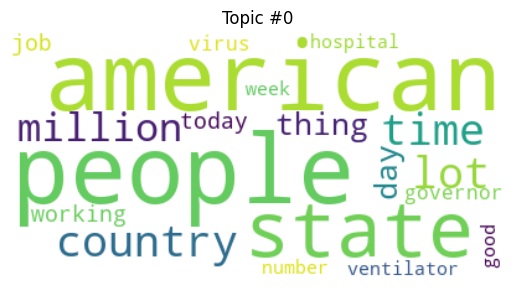
\includegraphics[scale=0.8]{output.png}
    \caption{Output of LDA: topic 0}
    \label{fig:lda}
\end{figure}
\begin{figure}
    \centering
    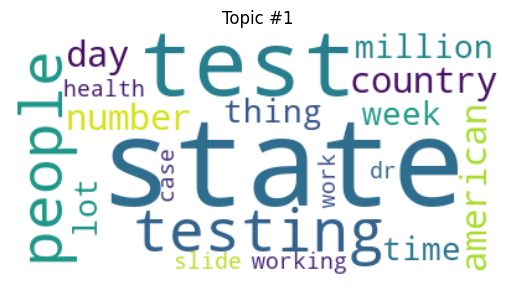
\includegraphics[scale=0.8]{output1.png}
    \caption{Output of LDA: topic 1}
    \label{fig:lda1}
\end{figure}
\begin{figure}
    \centering
    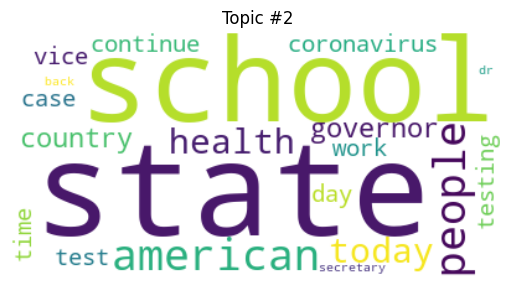
\includegraphics[scale=0.8]{output2.png}
    \caption{Output of LDA: topic 2}
    \label{fig:lda2}
\end{figure}


The Latent Dirichlet Allocation (LDA) algorithm was applied to the transcripts of speeches from the White House during the Trump administration. The resulting topics and their prominent keywords are as follows:

\begin{itemize}
    \item \textbf{Topic 0:} People, American, state, country, lot, time, million, thing, day, working, job, today, like, governor, virus, hospital, number, good, ventilator, week.
    
    \item \textbf{Topic 1:} State, test, testing, people, country, American, day, number, like, million, time, week, thing, lot, working, case, work, health, Dr., slide.
    
    \item \textbf{Topic 2:} State, school, American, people, today, health, governor, country, coronavirus, vice, case, time, continue, test, testing, work, day, secretary, back, Dr.
\end{itemize}

From these results, it becomes evident that the primary topics discussed during the Trump administration encompassed the following aspects:

\begin{itemize}
    \item \textbf{Topic 0:} Emphasis on the job market, economy, and healthcare, with mentions of hospitals and ventilators in the context of the COVID-19 pandemic.
    
    \item \textbf{Topic 1:} Focus on COVID-19 testing and cases, including discussions about health and work-related matters.
    
    \item \textbf{Topic 2:} Exploration of education and healthcare policies, involving mentions of governors and vice presidents.
\end{itemize}

\par

Additionally, grammar analysis was conducted to gain deeper insights into the linguistic features of the speeches. \newline Specific programs (\texttt{5\_a\_preprocessing\_for\_grammar.py}, \texttt{5\_b\_grammar\_tool.py}, and \texttt{5\_c\_fromtxttocsv.py}) were utilized to prepare the data for processing by the Cohmetrix software. 
The AI-driven Cohmetrix software facilitated the extraction of grammar-related metrics, which were then merged with the main dataset to provide a comprehensive linguistic analysis.
In-depth, these programs leverage AI models to autonomously process text through a web client platform. However, due to the intermittent unavailability of the Cohmetrix platform, we managed to procure grammar indices for only 68 records. To expand the analysis to encompass a larger dataset, the sequential execution of two programs is necessary: firstly, the execution of \texttt{5\_b\_grammar\_tool.py}, and subsequently, \texttt{5\_c\_fromtxttocsv.py}. These programs amalgamate the generated output files in txt format with our existing dataset.

\subsection{Statistical Modeling and Analysis}

The fourth stage entailed the application of sophisticated statistical modeling techniques to delve into the intricate interplay among speech sentiment, media dynamics, and financial market trends. I skillfully employed Structural Vector Autoregression (SVAR) and Vector Autoregression (VAR) models to scrutinize the potential determinants of uncertainty policy indices and their ramifications on economic indicators. The outcomes of the MATLAB-based VAR computations were systematically stored in the designated \texttt{VAR} directory, facilitating subsequent thorough analysis.
\par
It is important to highlight that this phase is presently under active development. The construction of a comprehensive SVAR and the extraction of insightful information necessitate a more extensive dataset. Unfortunately, the current scope of 68 records poses limitations. Our focus is on expanding the dataset to achieve a more robust analysis; however, the feasibility of this endeavor is contingent upon the availability of the Cohmetrix platform, which is under the jurisdiction of Memphis University. As such, our future progress in this avenue relies on collaborative efforts and external factors.

\subsection{Final remarks}

As a Research Assistant (RA) in this project, I underwent significant personal growth and skill development. Engaging in data collection refined my data management abilities, while delving into sentiment analysis with NLP models like BERT expanded my proficiency in language analysis. Applying advanced statistical models like SVAR and VAR deepened my understanding of economic interactions.
\par
I extend my heartfelt gratitude to my esteemed professor, \href{https://scholar.google.it/citations?user=noRmx74AAAAJ&hl=en}{Catalin Dragomirescu-Gaina}, whose unwavering support, guidance, and mentorship have been invaluable throughout this endeavor. Their insights and encouragement have played a pivotal role in shaping the trajectory of this research.
\par
In this process, I learned the importance of critical analysis and continuous improvement. While the project exhibited strengths, I identified areas for refinement, such as grammar analysis and sentiment modeling. Addressing these aspects not only enhanced the project's outcomes but also honed my analytical and problem-solving skills.
\par
Overall, my experience as an RA extended beyond project objectives, fostering personal growth and equipping me with valuable skills in data management, NLP, and statistical modeling. This journey has been instrumental in shaping my understanding of the intricate relationship between language, economics, and technology. My heartfelt appreciation goes to \href{https://scholar.google.it/citations?user=noRmx74AAAAJ&hl=en}{Catalin Dragomirescu-Gaina} for their instrumental role in this transformative experience.
\section{Additional materials}
All the materials of the RA is in the following github \href{https://github.com/RickyJ99/RA-project}{repository}.
\medskip

\bibliographystyle{plain}
\bibliography{references}

\end{document}
